\documentclass{beamer}
\usepackage[utf8]{inputenc}
\usepackage[style=apa, backend=biber]{biblatex}
\addbibresource{../../paper/bib.bib}
\usepackage{adjustbox}
\usepackage{booktabs}
\usepackage{siunitx}
\usepackage{amsmath}
\usepackage{amssymb}
\usepackage{amsthm}
\usepackage{yhmath}
\newcolumntype{d}{S[
	input-open-uncertainty=,
	input-close-uncertainty=,
	parse-numbers = false,
	table-align-text-pre=false,
	table-align-text-post=false
	]}

\usepackage{mathtext} 				% русские буквы в формулах
%\usepackage[T2A]{fontenc}			% кодировка
%\usepackage[utf8]{inputenc}			% кодировка исходного текста
\usepackage[english]{babel}	% локализация и переносы
\usepackage{changepage}
\usepackage{mathtools}


\usetheme{boxes}
\usecolortheme{default}

\setbeamertemplate{caption}{\insertcaption}
\setbeamertemplate{enumerate items}[circle]
\setbeamertemplate{itemize items}[circle]
\setbeamerfont*{frametitle}{size=\large}

% Title page details
\title[Social network in victim crime reporting]{Releasing the gatekeeper from duty:\\the role of social network\\in victim crime reporting}
%\subtitle{Quick-start guide}
\author[Bondarkov]{Sergey Bondarkov}
\institute[IRL]{Institute for the Rule of Law, EUSPb}
\date{\today}

\newcommand\citep{
	\parencite
}
\newcommand\citet{
	\textcite
}
\newcommand*{\tabindent}{\hspace{1em}}

\begin{document}
	
	% Title page
	\begin{frame}
		\titlepage
	\end{frame}
	
%	% Presentation outline
%	\begin{frame}{Outline}
%		\tableofcontents
%	\end{frame}
	
	% ==================================================================
	
	\section{Introduction}
	\subsection{From \textit{gatekeepers} to \textit{help-seekers}}
	\begin{frame}{Introduction: From \textit{gatekeepers} to \textit{help-seekers}}
		\begin{itemize}
			\item Any victimization is known to be unexpected and cause stress and confusion\citep{janoff1986aftermath}.
			\item A victim of crime is expected to turn to others in order `to reduce their uncertainty and be reassured'\citep{ruback1984social}. 
			\item I aim to make case for reframing reporting as a social process rather than an individual decision, \textit{à la}\citet{pescosolido1992beyond}. 
			\begin{itemize}
				\item Hence, a victim is redefined: from \textit{gatekeeper} \citep{gottfredson1987decision} who's primary function is to trigger the criminal justice system --- to \textit{help-seeker} who can take multiple paths in navigating the aftermath of victimization.
			\end{itemize}
			\item I show that activation of one's social network affects the path one takes in help-seeking: notifying the police becomes much more likely. 
		\end{itemize}
	\end{frame}	

	\subsection{Missing the social, or the data--theory feedback loop}
	\begin{frame}{Introduction: Missing the social, or the data--theory feedback loop}
		\begin{itemize}
			\item  While often overlooked, the importance of social network in victim crime reporting is not unrecognized\citep{bergemann2024social}.
			\item However, most of the work on the subject was focused on sexualized assault and intimate partner violence\citep{baert2024factors}, evidence for other types of crime remaining scarce\citep{xie2019crime}.
			\item As\citet{knoth2019reporting} put it, `\textit{studies that assess differences between individuals who report to the police, seek alternative help, or do nothing [...] often fail to recognize that individuals who do end up calling the police are likely to first seek advice from a third party}'.
		\end{itemize}
	\end{frame}	

	\begin{frame}{Introduction: Missing the social, or the data--theory feedback loop}
		\begin{itemize}
			\item Crime victimization surveys were designed to assess the dark figure of crime. They captured:
			\begin{itemize}
				\item features of an incident,
				\item features of a victim,
				\item if the crime was reported to the police.
			\end{itemize}
			\item Early studies found that reporting was strongly associated with \textit{seriousness} of crime and implied \textit{cost--benefit} calculation behind the decision to report\citep{skogan1984reporting}.
			\item They also found only mixed evidence of importance of a victim's \textit{demographics} and \textit{attitudes towards the police} --- being counterintuitive, this summoned more research focusing on these features.
			\item Thus, the quantitative research remained constrained to the original conceptual scope and the \textit{entrepreneur} metaphor.
		\end{itemize}
	\end{frame}	

	\begin{frame}{Introduction: Missing the social, or the data--theory feedback loop}
		\begin{itemize}
			\item Interestingly, the very paper by\citet{skogan1984reporting} that serves as \textit{the} reference for \textit{cost--benefit} perspective has already been touching on the \textit{role of others}.
			\item I speculate that it did not catch on mainly because there was no such dimension in the widely used victimization surveys\citep{xie2019crime}:
			\begin{itemize}
				\item In NCVS, a question about informing some party other than the police first appeared only in the latest update \citep{bjs@redesign}, the transition to the new instrument happened in 2025, the data is yet to be published. 
				\item In CSEW such question is reserved for 10-15 year-olds only.
				\item ICVS never featured such question.
			\end{itemize}
			\item Enter RCVS, which has included a question about informing friends and family right from the start (2018).
		\end{itemize}
	\end{frame}	

	\section{Data}
	\begin{frame}{Data}
		\begin{itemize}
			\item I use pooled data from three waves of the Russian Crime Victimization Survey (RCVS) \citep{kuchakov2026rcvs} ---  a nationally representative survey targeting the entire adult (18+) population of Russia.
			\item The survey waves were carried out in 2018, 2021, and 2024 in the Russian language. 
			\item All three survey waves employed a Random Digit Dialing (RDD) methodology --- a probability sampling technique in which telephone numbers are generated at random. Data collection was conducted using the Computer-Assisted Telephone Interviewing (CATI) method. 
			\item Raking algorithm was used to obtain weights for correction of sample imbalances.
		\end{itemize}
	\end{frame}

	\begin{frame}{Data}
		\begin{itemize}
			\item All respondents are asked only about their most recent incident occurring within the five years. 
			\item The type of an incident is derived from responses to a number of dichotomous questions presented in everyday language.
			\item After removing non-victims, victims of attempted cybercrime, and of offenses classified as `other', my sample consists of 5,697 observations.
			\item 	The questionnaires employed across the three waves are nearly identical.
			An exception important for this study is the question about \textit{emotional impact} of victimization --- it was introduced only in the 2024 wave. 
		\end{itemize}
	\end{frame}
	
	\begin{frame}{Data: Tabulation of reported cases share by principal variables}
		\begin{columns}
			\column{\dimexpr\paperwidth-10pt}
			\begin{adjustbox}{width=1\textwidth}
				\begin{tabular}{llrrrrrrrrrr}
					\toprule
					&  & \multicolumn{2}{c}{Cybercrime    } & \multicolumn{2}{c}{Fraud    } & \multicolumn{2}{c}{Theft    } & \multicolumn{2}{c}{Assault    } & \multicolumn{2}{c}{Robbery} \\ 
					\cmidrule(lr){3-4} \cmidrule(lr){5-6} \cmidrule(lr){7-8} \cmidrule(lr){9-10} \cmidrule(lr){11-12}
					&     & N & Rep. (SE) & N  & Rep. (SE)  & N   & Rep. (SE)   & N    & Rep. (SE)    & N     & Rep. (SE)     \\ 
					\multicolumn{12}{l}{\textsc{Totals}} \\
					Survey wave & 2018 & 442 & 0.43 (0.04) & 328 & 0.38 (0.04) & 841 & 0.62 (0.03) & 211 & 0.53 (0.05) & 141 & 0.73 (0.06) \\ 
					& 2021 & 837 & 0.44 (0.02) & 208 & 0.53 (0.05) & 545 & 0.62 (0.03) & 266 & 0.59 (0.04) & 100 & 0.68 (0.06) \\ 
					& 2024 & 695 & 0.52 (0.02) & 34 & 0.73 (0.11) & 394 & 0.56 (0.03) & 254 & 0.56 (0.04) & 78 & 0.62 (0.07) \\ 
					& Pooled & 1974 & 0.47 (0.02) & 570 & 0.45 (0.03) & 1780 & 0.61 (0.02) & 731 & 0.56 (0.02) & 319 & 0.69 (0.04) \\ 
					\midrule
					\multicolumn{12}{l}{\textsc{Post-victimization behavior}} \\
					% \addlinespace[4pt]
					Victim informed %friends or relatives 
					& No & 305 & 0.36 (0.04) & 58 & 0.31 (0.09) & 118 & 0.42 (0.06) & 129 & 0.2 (0.05) & 42 & 0.46 (0.13) \\ 
					friends or relatives  & Yes & 1669 & 0.49 (0.02) & 512 & 0.47 (0.03) & 1662 & 0.62 (0.02) & 602 & 0.65 (0.03) & 277 & 0.71 (0.04) \\ 
					\vspace{1pt}\\
					Victim went & No & 1974 & 0.47 (0.02) & 570 & 0.45 (0.03) & 1780 & 0.61 (0.02) & 385 & 0.41 (0.03) & 187 & 0.64 (0.05) \\ 
					to hospital & Yes & 0 & n/a & 0 & n/a & 0 & n/a & 346 & 0.74 (0.03) & 132 & 0.77 (0.05) \\ 
					\midrule
							\multicolumn{12}{l}{\textsc{Incident characteristics}} \\
					% \addlinespace[4pt]
					Damage: money,& 0 to 1 & 185 & 0.22 (0.04) & 48 & 0.24 (0.09) & 191 & 0.49 (0.05) & 555 & 0.52 (0.03) & 39 & 0.61 (0.11) \\ 
					thnd rub. & 1 to 10 & 702 & 0.31 (0.02) & 118 & 0.26 (0.06) & 423 & 0.45 (0.03) & 67 & 0.59 (0.07) & 62 & 0.61 (0.09) \\ 
					& 10 to 50 & 561 & 0.5 (0.03) & 137 & 0.39 (0.06) & 636 & 0.61 (0.03) & 46 & 0.7 (0.09) & 116 & 0.66 (0.06) \\ 
					& 50+ & 526 & 0.7 (0.03) & 267 & 0.65 (0.04) & 530 & 0.76 (0.03) & 63 & 0.85 (0.06) & 102 & 0.78 (0.06) \\ 
					\vspace{1pt}\\
					Damage: physical & No & 0 & n/a & 0 & n/a & 0 & n/a & 175 & 0.44 (0.05) & 53 & 0.6 (0.09) \\ 
					& Light & 0 & n/a & 0 & n/a & 0 & n/a & 246 & 0.5 (0.04) & 83 & 0.69 (0.08) \\ 
					& Heavy & 0 & n/a & 0 & n/a & 0 & n/a & 134 & 0.74 (0.05) & 58 & 0.67 (0.08) \\ 
					\vspace{1pt}\\
					Damage: emotional & Light & 129 & 0.33 (0.05) & 4 & 0.75 (0.34) & 75 & 0.47 (0.07) & 56 & 0.37 (0.08) & 4 & 0.75 (0.39) \\ 
					(wave 2024 only) & Medium & 167 & 0.48 (0.05) & 6 & 0.05 (0.17) & 109 & 0.61 (0.06) & 55 & 0.46 (0.08) & 22 & 0.44 (0.12) \\ 
					& Heavy & 393 & 0.58 (0.03) & 24 & 0.96 (0.05) & 206 & 0.56 (0.04) & 143 & 0.67 (0.05) & 52 & 0.67 (0.08) \\ 
					\bottomrule
					\vspace{1pt}\\
					\multicolumn{12}{l}{\small Proportions of reported victimizations and standard errors were calculated using observations' weights to correct for sample imbalances.}
				\end{tabular}
			\end{adjustbox}
		\end{columns}
	\end{frame}
		
	\section{Methods}
	\begin{frame}{Methods: Framework}
		Individual-level: decision making model developed in \textit{After the Crime} by\citet{greenberg1992after}:
			\begin{itemize}
				\item a victim is stressed, their assumptions about the world challenged,
				\item they may need help to
				\begin{itemize}
					\item label the incident as crime, 
					\item assess its seriousness, 
					\item think through response options;
				\end{itemize} 
				\item others' influence takes form of 
				\begin{itemize}
					\item cuing the victim to particular options and scripts not yet considered,
					\item providing information, 
					\item channeling certain norms, 
					\item offering emotional and practical support.  
				\end{itemize}
			\end{itemize}		
	\end{frame}

	\begin{frame}{Methods: Framework}
		Network-level: help-seeking as a social process, in the spirit of\citet{pescosolido1992beyond}:
		\begin{itemize}
			\item social phenomena occurs in interaction, rather than in isolated cost--benefit driven decisions,
%			\item victimization emerge as a shock not only to an individual but to a broader network, 
			\item we should focus on these interactions, i.e. on the paths people take in seeking help,
			\item response, such as reporting to the police, emerge on these paths,
			\item the principal question, then, is what defines these paths.
		\end{itemize}		
		
		I aim to make case for this perspective by
		\begin{itemize}
			\item showing how social network activation affects path (probability of passing through the police station),
			\item exploring predictors of social network activation.
		\end{itemize}
	
	\end{frame}

	\begin{frame}{Methods: Model}
		\begin{figure}
			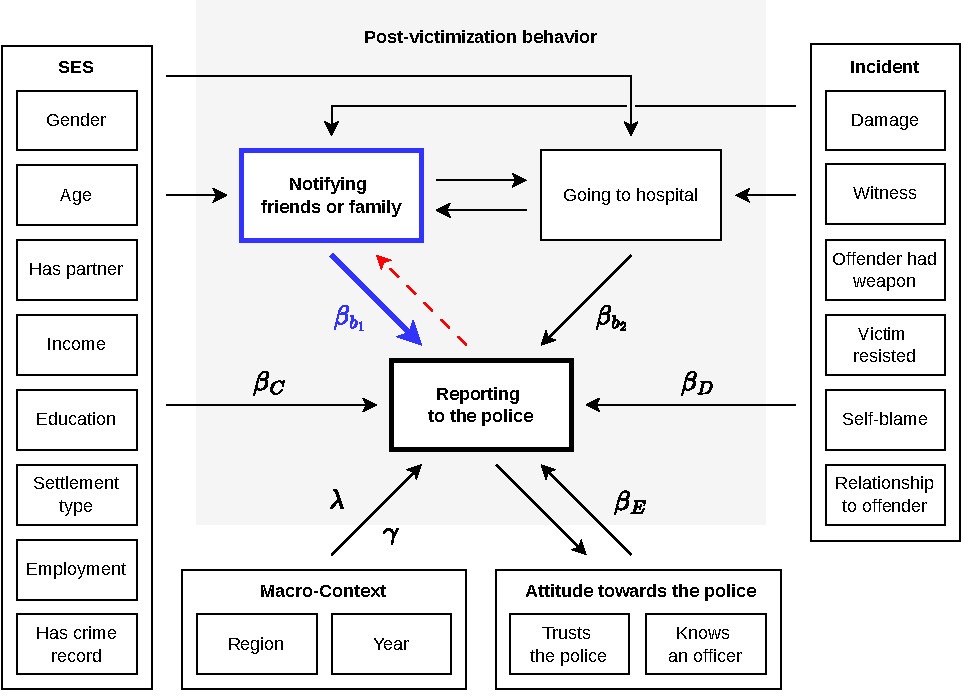
\includegraphics[width = 1\textwidth]{../../paper/figures/causal_diagram_color.pdf}
		\end{figure}		
	\end{frame}

	\begin{frame}{Methods: Model}
		My base model has the following linear form:
		\vspace{-1pt}
		\begin{equation}
			\begin{multlined}[0.9\linewidth]
				\small
%				\label{eq:1}
				Reported_i = \beta_{b_1} ToldSomeone_i + \beta_{b_2} WentHospital_i\\\nonumber + \sum \beta_C SES_i + \sum \beta_D Incident_i + \sum \beta_E Attitude_i + \lambda_i + \gamma_i + \epsilon_i
			\end{multlined}
		\end{equation}
		where 
		\begin{itemize}
			\small
			\item $Reported$ is a binary indicator of informing the police, 
			\item $ToldSomeone$ indicates if a victim talked with friends or family about the incident,
			\item $WentHospital$ indicates seeking medical help,
			\item $SES$ comprises variables related to socioeconomic status,
			\item $Incident$ stands for incident characteristics,
			\item $Attitude$ is a vector of variables that capture a victim's attitude towards the police,
			\item $\lambda$ and $\gamma$ are region and survey year fixed effects.
		\end{itemize}
		
	\end{frame}

	\begin{frame}{Methods: Model}
		I estimate the model using logistic regression. Since post-victimization behavior is known to vary with crime type\citep{greenberg1992after}, I run separate regressions on six subsets of data split by crime type: 
		\begin{itemize}
			\item theft,
			\item face-to-face fraud,
			\item cybercrime,
			\item assault,
			\item all property crime, 
			\item all violent crime.
		\end{itemize} 
	
		Property crime comprises theft, fraud, and cybercrime; violent crime includes assault and robbery (the latter being too rare to estimate a separate model).		
	\end{frame}
	
	\section{Results}
	\begin{frame}{\small Results 1: Odds ratios of reporting (abbr. regression table)}
		\begin{columns}
			\column{\dimexpr\paperwidth-20pt}
			\centering
			\begin{adjustbox}{width=.85\textwidth}

				\begin{tabular}{@{\hspace*{1.5em}}lS[table-format=1.3]@{\hspace{1cm}}S[table-format=1.3]S[table-format=1.3]S[table-format=1.3]S[table-format=1.3]S[table-format=1.3]S[table-format=1.3]}
					
					\toprule
					& {Theft} & {Fraud} & {Cybercrime} & {Assault} & {All prop.} & {All viol.} \\ 
					\midrule\addlinespace[2.5pt]
					\multicolumn{7}{l}{\textsc{Post-victimization behavior}} \\
					Victim informed friends or family & 2.407*** & 1.769 & 1.898** & 8.203*** & 2.121*** & 10.335*** \\ 
					Victim went to hospital &  &  &  & 12.422*** &  & 10.743*** \\ 
%					\multicolumn{7}{l}{\textsc{Socioeconomic status}} \\
%					Male & 0.730 & 0.834 & 0.871 & 0.593 & 0.851*** & 0.580 \\ 
%					Age (\textit{ref. level}: 35--49):\\
%					\tabindent 18--24 & 0.242*** & 4.000* & 0.690{+} & 0.202{+} & 0.530*** & 0.280{+} \\ 
%					\tabindent 25--34 & 0.731 & 0.491{+} & 0.832 & 0.398{+} & 0.758* & 0.598 \\ 
%					\tabindent 50--64 & 0.560* & 0.679 & 0.740 & 0.736 & 0.704*** & 1.289 \\ 
%					\tabindent 65{+} & 1.194 & 0.257{+} & 1.052 & 4.446 & 0.961 & 2.946 \\
					\multicolumn{7}{l}{\textsc{Incident characteristics}} \\
					Damage:\\
					\multicolumn{7}{l}{\hspace*{2em}Financial, thnd rub. (\textit{ref. level}: 0 to 1):}\\
					\tabindent\tabindent 1 to 10 & 0.842 & 0.990 & 1.872* & 2.086 & 1.189 & 1.835 \\ 
					\tabindent\tabindent 10 to 50 & 1.929*** & 1.884 & 4.126*** & 3.107 & 2.561*** & 2.583*** \\ 
					\tabindent\tabindent 50$+$ & 3.768*** & 7.830*** & 10.477*** & 4.241*** & 5.626*** & 2.954*** \\  
					\tabindent Physical (\textit{ref. level}: No):\\
					\tabindent\tabindent Light &  &  &  & 1.014 &  & 1.167 \\ 
					\tabindent\tabindent Heavy &  &  &  & 1.453 &  & 0.897 \\ 
					There was a witness &  &  &  & 1.749 &  & 1.196 \\ 
					Victim resisted &  &  &  & 0.689 &  & 0.516 \\ 
					Offender had a weapon &  &  &  & 2.024** &  & 1.961 \\ 
					Self-blame & 0.548*** & 0.822 & 0.511*** & 0.823 & 0.533*** & 0.565** \\  
					\multicolumn{7}{l}{\hspace*{1em}Victim-offender relationship (\textit{ref. level}: Stranger):}\\
					\tabindent Acquaintance &  &  &  & 1.186 &  & 0.914 \\ 
					\tabindent Colleague or neighbor &  &  &  & 6.790** &  & 11.795*\\ 
					\tabindent Friend or relative &  &  &  & 0.457 &  & 0.733 \\ 
					\tabindent Spouse or partner &  &  &  & 0.691 &  & 1.050 \\ 
					\midrule
					N & {1752} & {518} & {1959} & {463} & {4308} & {628} \\ 
					McFaddens' R2 & 0.202 & 0.328 & 0.188 & 0.500 & 0.157 & 0.452 \\ 
					\bottomrule 
					\addlinespace[2.5pt]
					\multicolumn{7}{l}{\footnotesize * $p < 0.1$, ** $p < 0.05$, *** $p < 0.01$. All models include controls for demographics variables and attitude proxies,}\\
					\multicolumn{7}{l}{\footnotesize as well as region and survey year FE. Standard errors are clustered by region and survey year. Observations' weights are}\\
					\multicolumn{7}{l}{\footnotesize used to correct sample imbalances.}\\
				\end{tabular}
				\end{adjustbox}
			
			\end{columns}
		\end{frame}
	
	\begin{frame}{\small Results 1: Robustness tests (odds ratios of reporting, abbr. regression tables)}
		\begin{columns}
			\column{\dimexpr\paperwidth-20pt}
			\centering
			\begin{adjustbox}{width=.85\textwidth}
				\begin{tabular}{@{\hspace*{1.5em}}lS[table-format=1.3]@{\hspace{1cm}}S[table-format=1.3]S[table-format=1.3]S[table-format=1.3]S[table-format=1.3]S[table-format=1.3]}	
					\toprule
					& {Theft} & {Fraud} & {Cybercrime} & {Assault} & {All prop.} & {All viol.} \\ 
					\midrule\addlinespace[2pt]
					\multicolumn{7}{l}{\textsc{Panel A. Base model, pooled data of three survey waves}} \\
					\addlinespace[2.5pt]
					Victim informed friends or family & 2.407*** & 1.769 & 1.898** & 8.203*** & 2.121*** & 10.335*** \\ 
					\addlinespace[10pt]
					N & {1752} & {518} & {1959} & {463} & {4308} & {628} \\ 
					McFaddens' R2  & 0.202 & 0.328 & 0.188 & 0.500 & 0.157 & 0.452 \\  
					\addlinespace[10pt]
					\multicolumn{7}{l}{\textsc{Panel B. Base model, wave 2024 only}} \\
					\addlinespace[2.5pt]
					{Victim informed friends or family} & {2.516} &  & {1.491} & {23.997***} & {1.598*} & {23.520**} \\ 
					\addlinespace[10pt]
					N & {328} & & {665} & {186} & {1082} & {229} \\ 
					McFaddens' R2 & 0.266 & & 0.199 & 0.623 & 0.171 & 0.613 \\ 
					\addlinespace[10pt]
					\multicolumn{7}{l}{\textsc{Panel C. Base model augmented with emotional damage, wave 2024 only}} \\
					\addlinespace[2.5pt]
					Victim informed friends or family & 2.511 & & 1.442 & 20.065** & 1.552* & 21.506** \\ 
					\multicolumn{7}{l}{\hspace{1em}Emotional damage (\textit{ref. level}: Light):}\\
					\tabindent Medium & 1.473 & & 1.605 & 1.610 & 1.359 & 1.413 \\ 
					\tabindent Heavy & {1.515} & & {1.811} & {0.745} & {1.735*} & {0.541} \\ 
					\addlinespace[10pt]
					N & {324} & & {657} & {186} & {1072} & {229} \\ 
					McFaddens' R2 & 0.261 & & 0.199 & 0.621 & 0.170 & 0.613 \\ 
					\addlinespace[10pt]
					\multicolumn{7}{l}{\textsc{Panel D. Base model, pooled data, reported-but-no-case observations removed}} \\
					\addlinespace[2.5pt]
					Victim informed friends or family & 2.485*** & 1.289 & 1.304 & 16.080** & 1.837 & 23.570*** \\ 
					\addlinespace[10pt]
					N &  {1234} & {323} & {1478} & {281} & {3150} & {403} \\
					McFaddens' R2 & 0.254 & 0.419 & 0.251 & 0.625 & 0.206 & 0.556 \\
					\bottomrule
					\addlinespace[2.5pt]
					\multicolumn{7}{l}{\footnotesize * $p < 0.1$, ** $p < 0.05$, *** $p < 0.01$. All models include controls for demographics variables, incident  features, and attitude}\\
					\multicolumn{7}{l}{\footnotesize proxies. FE are region and year in panel A and D, region only in panels B and C. Standard errors are clustered by region}\\
					\multicolumn{7}{l}{\footnotesize and year in panels A and D, by region only in panels B and C. Observations' weights are used to correct sample imbalances.}\\
%					\multicolumn{7}{l}{\footnotesize Observations' weights are used to correct sample imbalances.}\\
%					\multicolumn{7}{l}{}\\
					%	\multicolumn{6}{l}{All models include the same list of control variables, fixed effects are region and year in panel A and D, region only in panels B and C. Standard errors are clustered by region and year in panels A and D, by region only in panels B and C.}
				\end{tabular}
			\end{adjustbox}
		\end{columns}
	\end{frame}

	\begin{frame}{\small Results 2: Odds ratios of social network activation}
		\begin{columns}
			\column{\dimexpr\paperwidth-20pt}
			\centering
			\begin{adjustbox}{width=.85\textwidth}
				\begin{tabular}{@{\hspace*{1.5em}}lS[table-format=1.3]@{\hspace{1cm}}S[table-format=1.3]S[table-format=1.3]S[table-format=1.3]S[table-format=1.3]S[table-format=1.3]S[table-format=1.3]}
					
					\toprule
					& {Theft} & {Fraud} & {Cybercrime} & {Assault} & {All prop.} & {All viol.} \\ 
					\midrule\addlinespace[2.5pt]
%					\multicolumn{7}{l}{\textsc{Post-victimization behavior}} \\
%					Victim went to hospital &  &  &  & 2.915* &  & 2.325* \\ 
					\multicolumn{7}{l}{\textsc{Socioeconomic status}} \\
					Male & 0.448*** & 0.227* & 0.401*** & 0.436 & 0.476*** & 0.450 \\ 
					Age (\textit{ref. level}: 35--49):\\
					\tabindent 18--24 & 0.679 & 1.019 & 1.479 & 0.299** & 0.995 & 0.403* \\ 
					\tabindent 25--34 & 0.554 & 2.112** & 1.319 & 0.173*** & 0.899 & 0.232*** \\ 
					\tabindent 50--64 & 1.031 & 1.474 & 1.209 & 1.546 & 0.974 & 2.124 \\ 
					\tabindent 65{+} & 0.637 & 0.777 & 1.152 & 0.943 & 0.788 & 1.639 \\ 
					Has a partner & 2.185** & 1.869 & 1.668* & 1.133 & 1.716** & 1.360 \\ 
					Middle to upper household income & 1.512** & 0.307** & 1.3508 & 0.844 & 1.075 & 0.905 \\ 
					Small town or village & 1.026 & 0.344 & 0.974 & 0.528 & 0.914 & 0.455** \\ 
					Higher education & 1.483* & 4.684 & 0.998 & 0.814 & 1.196 & 0.836 \\ 
					Employed or student & 0.957 & 1.227 & 1.806** & 1.803 & 1.299 & 1.920 \\ 
					\multicolumn{7}{l}{\textsc{Incident characteristics}} \\
					Self-blame & 0.623 & 0.910 & 0.667* & 1.220 & 0.589*** & 1.311 \\ 
					\multicolumn{7}{l}{\hspace*{1em}Victim-offender relationship (\textit{ref. level}: Stranger):}\\
					\tabindent Acquaintance &  &  &  & 0.091*** &  & 0.075*** \\ 
					\tabindent Colleague or neighbor &  &  &  & 1.730 &  & 1.595 \\ 
					\tabindent Friend or relative &  &  &  & 0.533 &  & 0.517 \\ 
					\tabindent Spouse or partner &  &  &  & 1.117 &  & 0.626 \\  
					%	\vspace{1pt}\\ 
					\multicolumn{7}{l}{\textsc{Victim's attitude towards the police}} \\
					Has crime record & 0.566 & 4.604 & 1.247 & 0.718 & 0.879 & 0.734 \\ 
					%	\vspace{1pt}\\
					{Knows an officer} & {1.067} & {5.667**} & {1.570**} & {0.501} & {1.415} & {0.755} \\   
					\midrule
					N & {1431} & {344} & {1895} & {416} & {4260} & {557} \\  
					McFaddens' R2 & 0.218 & 0.363 & 0.129 & 0.361 & 0.133 & 0.379 \\  
					%	Pseudo-R2 Within & 0.097 & 0.181 & 0.062 & 0.222 & 0.051 & 0.227 \\ 
%					FE: Region & X & X & X & X & X & X \\ 
%					FE: Survey year & X & X & X & X & X & X \\ 
					\bottomrule
					\addlinespace[2.5pt]
					\multicolumn{7}{l}{\footnotesize * $p < 0.1$, ** $p < 0.05$, *** $p < 0.01$. All models include controls for going to hospital, damage level, victim resistance,}\\
					\multicolumn{7}{l}{\footnotesize weapon use, witness presence, as well as region and survey year FE. Standard errors are clustered by region and survey year.}\\
					\multicolumn{7}{l}{\footnotesize  Observations' weights are used to correct sample imbalances.}\\
				\end{tabular}
			\end{adjustbox}
		\end{columns}
	\end{frame}

	\section{Conclusion}
	\begin{frame}{Conclusion}
	Activation of social network does affect the path of help-seeking after criminal victimization:
			\begin{itemize}
				\item the effect is more pronounced in violent crime, where it is as large as that of visiting hospital,
				\item in property crimes modeling results are mixed: 
				\begin{itemize}
					\item theft: the effect is fairly stable,
					\item face-to-face fraud: no effect,
					\item cybercrime: evidence is tentative.
				\end{itemize}
			\end{itemize}
	\end{frame}

	\begin{frame}{Conclusion}
		Turning to the intimate circle for help is strongly associated with demographics variables:
		\begin{itemize}
			 \item being a male is a prominent negative predictor of informing friends or family about property victimization,
			\item younger victims are much less likely to discuss violent victimization with others,
			\item having a partner makes sharing more probable in cases of theft and cybercrime but not fraud,
			\item higher household income is positively associated with the probability of discussing theft, but negatively in case of fraud,
			\item living in a small town or village halves chances of relating a story about violent victimization. 
		\end{itemize}
	\end{frame}

	\begin{frame}{Conclusion}
		Also, the character of victimization plays its role:
		\begin{itemize}
			\item cybercrime victimization seems to produce shame that precludes seeking help,
			\item violent victimization by an acquaintance is hard to share with the intimate circle.
		\end{itemize}
	\end{frame}

	\begin{frame}{Conclusion}
		These results warrant further exploration of post-victimization behavior from social interaction perspective:
		\begin{itemize}
			\item mapping paths people take in seeking help
			\item and studying factors of taking or of availability of these paths. 
		\end{itemize}
		
		This will require updating our instruments:
		\begin{itemize}
			\item we need to record the order of events post-victimization,
			\item we are should be interested in the content of the interactions along the path.
		\end{itemize} 

	\end{frame}
	
	



	\printbibliography %Prints bibliography
\end{document}